
\begin{frame}{\citetitle{Plagio_Marlly2022}$^*$  (1)}
\begin{columns}
\begin{column}{0.6\textwidth}
	\begin{itemize}
		\item El plagio es un común denominador en diferentes niveles educativos
        \item Se propone un sistema que analiza un conjunto de documentos y detecta plagio mediante diferentes enfoques:
		\begin{itemize}
		\item Analizar el texto de dichos documentos y compararlos entre sí
		\item Extraer y analizar las imágenes y compararlas entre sí
		\end{itemize}
	\end{itemize}
\end{column}
\begin{column}{0.4\textwidth}  
\begin{center}
     \begin{tabular}{c}
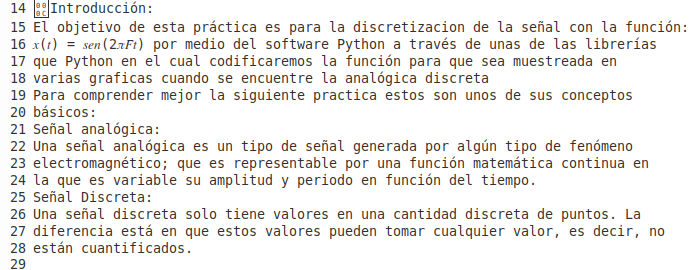
\includegraphics[width=0.78\textwidth]{2022_Plagio/figs/P1}\\ \hline
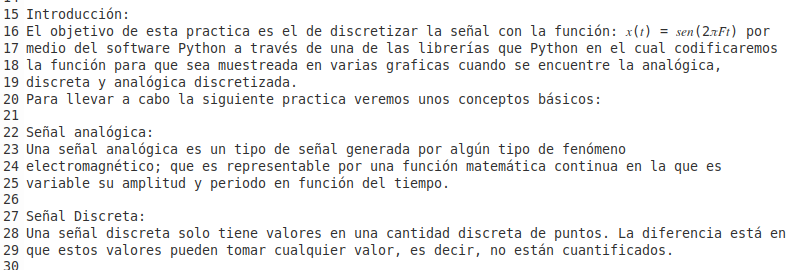
\includegraphics[width=0.78\textwidth]{2022_Plagio/figs/P2}\\         
      \end{tabular}
\end{center}
\end{column} 
\end{columns} 
\footfullcite*{Plagio_Marlly2022}
\end{frame}


\begin{frame}{\citetitle{Plagio_Marlly2022} (2)}
	\begin{itemize}
        \item La aplicación esta codificada en Python, hace uso de OpenCV para comparar imágenes y la librería \textit{TfidVectorizer} para comparación de textio
        \item Una vez efectuado el análisis, se reportan los resultados
	\end{itemize}
\begin{center}
 \begin{tabular}{c}
    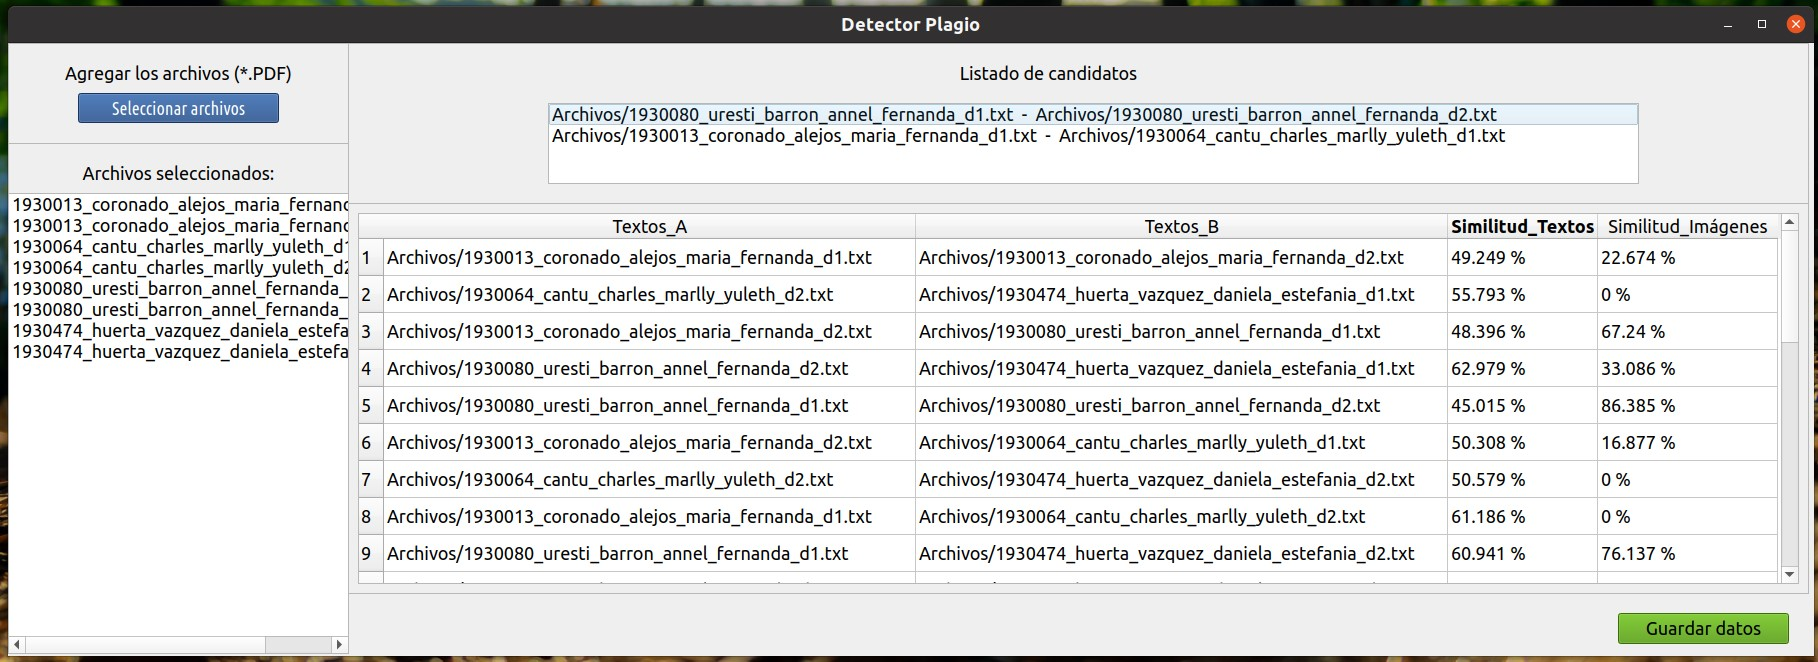
\includegraphics[width=0.64\textwidth]{2022_Plagio/figs/analisis.jpg}
  \end{tabular}
\end{center}

\end{frame}





